%\documentclass[handout]{beamer}
\documentclass{beamer}
\usepackage[utf8]{inputenc}
\usepackage[francais]{babel}
\usepackage[T1]{fontenc}
%\usepackage{multimedia}
\usepackage{graphicx}
\usepackage{hyperref}
\usepackage{algorithm}
\usepackage{algpseudocode}
\floatname{algorithm}{Algorithme} 
\usepackage{listings}

%\usetheme[width=100pt]{PaloAlto}
\usetheme[compress]{Ilmenau}
%\usecolortheme{fly}
\setbeamertemplate{frametitle}[default][center]

%\setbeamercovered{transparent}

\title{Proactive : Un middleware open source pour le calcul parallèle}

\author{Veyssier Julien}
\institute{CBGP - INRA}
\date{25 Octobre 2011}
\setbeamertemplate{navigation symbols}{}
%\logo{}
\begin{document}

\begin{frame}
\titlepage
\end{frame}

\begin{frame}
\tableofcontents
\end{frame}

\section[Introduction]{Introduction}
\begin{frame}
	\tableofcontents[currentsection]
\end{frame}

\begin{frame}{Contexte}
	\begin{columns}
	\begin{column}[l]{0.5\linewidth}
        \begin{columns}
        \begin{column}[l]{0.5\linewidth}
        \begin{figure}
            %[!bh]
            \centering
            
\includegraphics[scale=0.32]{cbgp.png}
            %\caption{Architecture autour d'un CDN}
        \end{figure}
        \end{column}
        \begin{column}[r]{0.5\linewidth}
        \begin{figure}
            %[!bh]
            \centering
            
\includegraphics[scale=0.32]{cocci.png}
            %\caption{Architecture autour d'un CDN}
        \end{figure}
        \end{column}
        \end{columns}
        \vspace{1cm}
	\begin{block}{Objectifs}<2->
			\begin{itemize}
                    %decouplage .. .
                \item Refonte de DIYABC
				\item Implémentation de l'interface graphique
                \item Interfaçage avec des outils de calcul parallèle
			\end{itemize}
					
		\end{block}

	\end{column}
	\begin{column}[r]{0.5\linewidth}
	\begin{exampleblock}{Activités du laboratoire}<1->
			\begin{itemize}
				\item Génétique des population
                \item Systématique
                \item Écologie
			\end{itemize}
					
		\end{exampleblock}
	\begin{block}{Moyens matériels}<3->
			\begin{itemize}
                \item Cluster local (SGE)
				\item Machines personnelles des chercheurs
                \item Postes de travail de l'administration
			\end{itemize}
					
		\end{block}
	\end{column}
	\end{columns}
\end{frame}

\begin{frame}{Exploration des alternatives à SGE}
    Constat : architectures trop rigides et fastidieuses à maintenir
	\begin{columns}
	\begin{column}[l]{0.3\linewidth}
    \begin{block}{Projets}
        \begin{itemize}
                % alex a utilisé diane, bien mais manque d'outils qui facilitent la vie
            \item<2-> Diane
                % sous partie de diane
            \item<3-> Ganga
                % orienté grilles
            \item<4-> Wisdom
                % example de projet qui ne fourni pas son programme
            \item<5-> OurGrid
            \item<6-> Proactive
        \end{itemize}
    \end{block}
	\end{column}
	\begin{column}[r]{0.6\linewidth}
    \begin{exampleblock}{Particularité}
        \begin{itemize}
            \item<2-> Peu d'outils annexe
            \item<3-> Sous-partie de DIANE
            \item<4-> Orienté vers les grilles de calcul
            \item<5-> Programmes non fournis
            \item<6-> Découplé et polyvalent
        \end{itemize}
    \end{exampleblock}
	\end{column}
	\end{columns}
\end{frame}

\begin{frame}{Proactive}
    Exploration des possibilités pour une éventuelle intégration au CBGP
\end{frame}

\section[Fonctionnement]{Fonctionnement de Proactive}
\begin{frame}{Caractéristiques}
    \begin{itemize}
        \item Langage de programmation $\Longrightarrow$ Java + Bash/Batch
        \item Portable
        \item Supporte un environnement hétérogène (Unix*, Windows)% scripts de selection
        \item Différents niveaux d'utilisation % simple, avancé
        \item Différentes interfaces : GUI, CLI, API (intégration dans votre propre application)
        \item Extensible et découplé
            % decouplé : chaque executable est indépendant et ne nécessite pas forcément l'exécution des autres
            % extensible : logiciel libre sous affero GPL que l'on peut améliorer
    \end{itemize}

\end{frame}
\subsection{Architecture}
\begin{frame}{Architecture}
	\begin{columns}
	\begin{column}[l]{0.5\linewidth}
        \begin{figure}
            %[!bh]
            \centering
            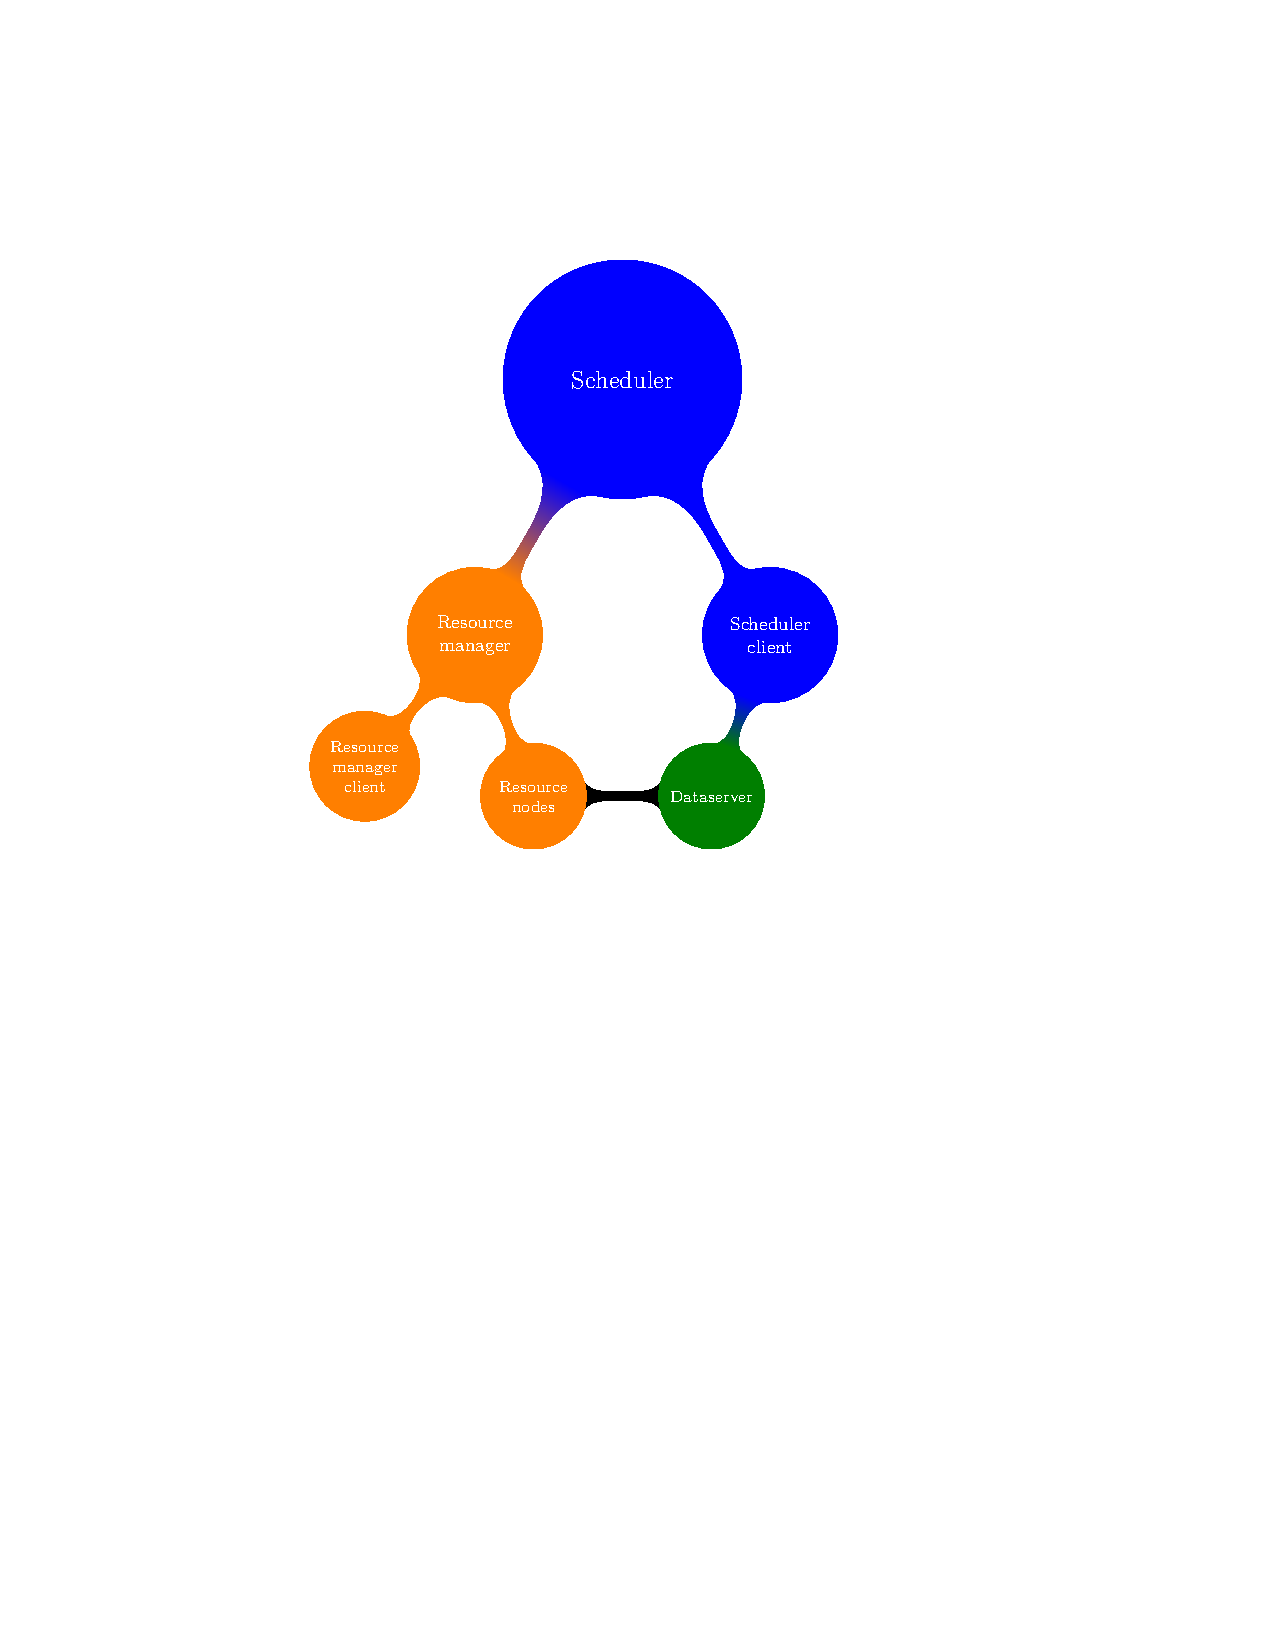
\includegraphics[trim=4cm 13cm 2cm 5cm,scale=0.48]{netmap_abs.pdf}
            \caption{Communication dans Proactive}
        \end{figure}
	\end{column}
    \setbeamercolor{block title}{fg=black,bg=orange}   
    \setbeamercolor{block body}{fg=black,bg=orange!30}
    \setbeamercolor{block title alerted}{fg=black,bg=blue}   
    \setbeamercolor{block body alerted}{fg=black,bg=blue!30}
    \setbeamercolor{block title example}{fg=black,bg=green!50!black}   
    \setbeamercolor{block body example}{fg=black,bg=green!15}
	\begin{column}[r]{0.5\linewidth}
        \begin{block}{Resource management}
            Gestion des noeuds de calcul
        \end{block}
        \begin{alertblock}{Scheduler}
             Gestion de la politique d'ordonnancement et de la soumission des t\^aches
        \end{alertblock}
        \begin{exampleblock}{Data management}
            Transmission des données
        \end{exampleblock}
        
	\end{column}
	\end{columns}
\end{frame}

\subsection{Composants}
\begin{frame}{Programmes}
	\begin{columns}
	\begin{column}[l]{0.5\linewidth}
        \begin{figure}
            %[!bh]
            \centering
            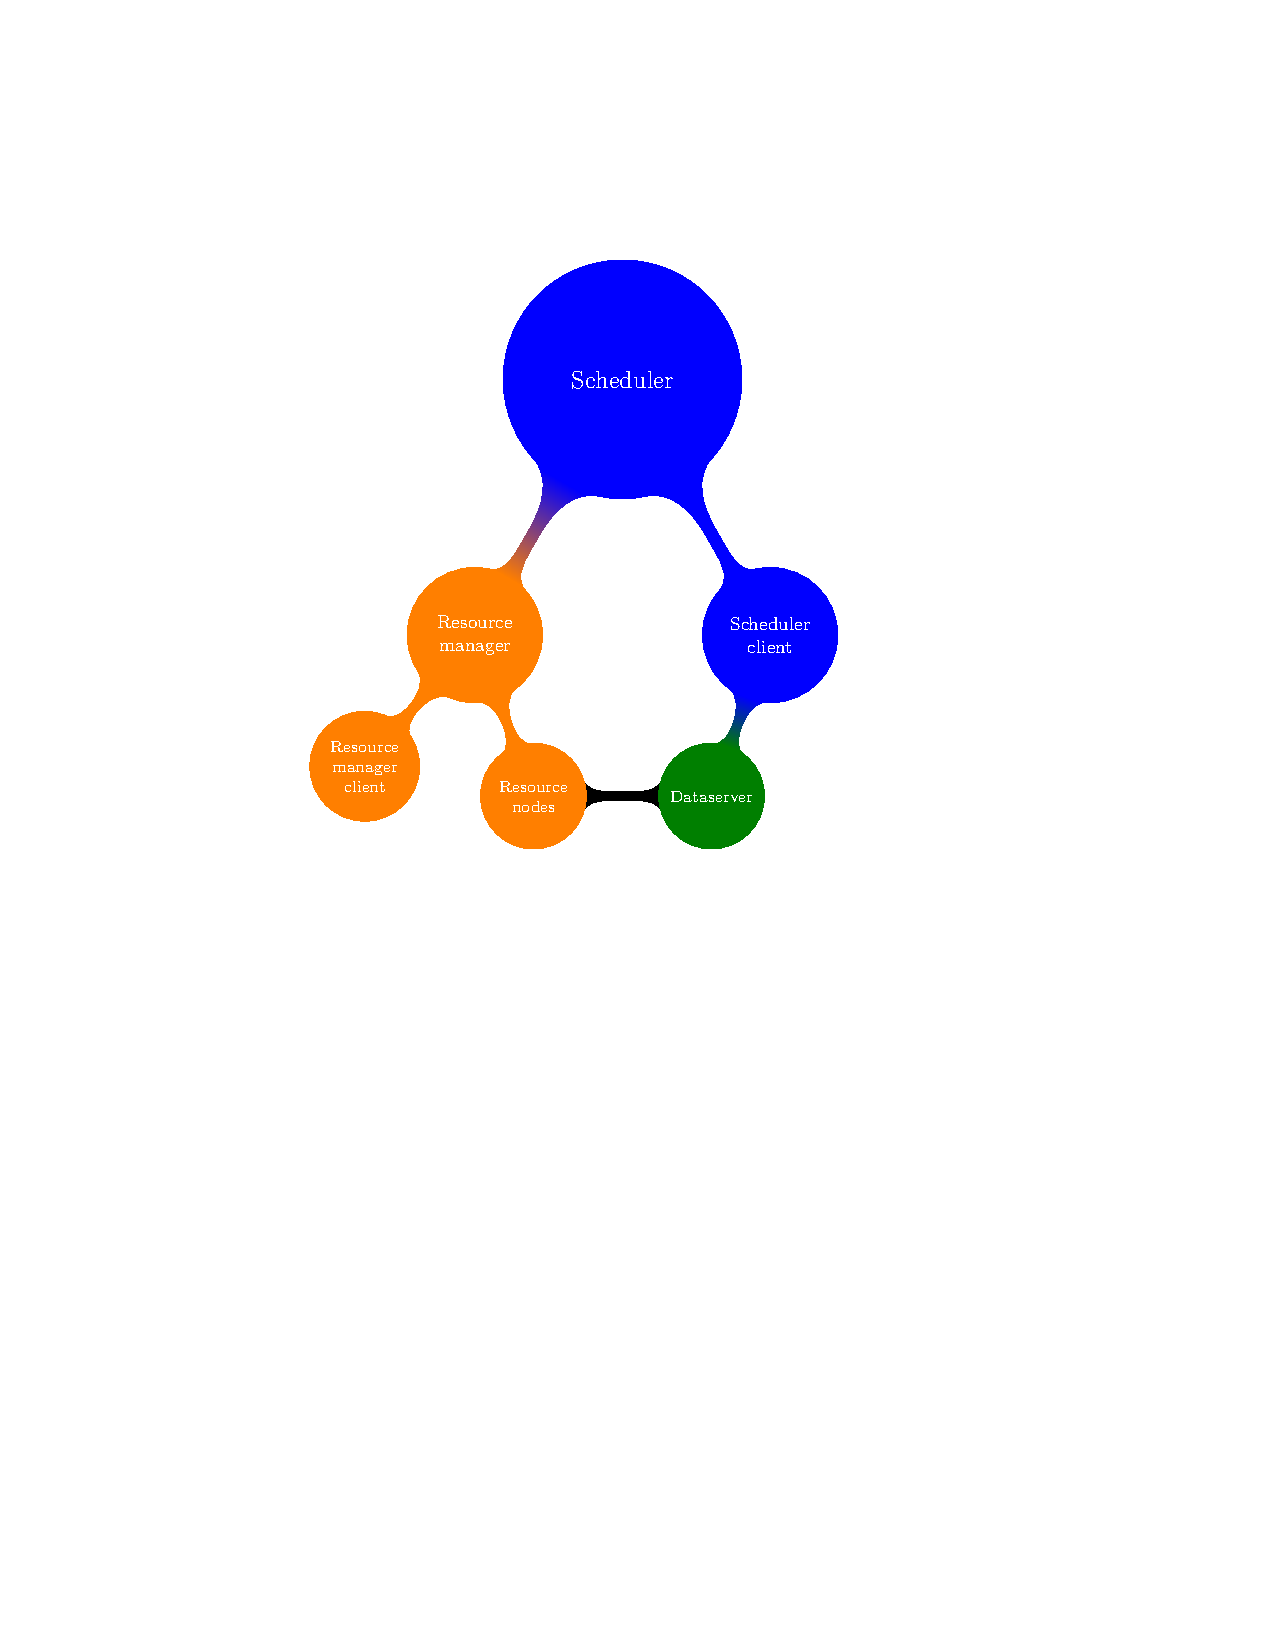
\includegraphics[trim=4cm 13cm 2cm 5cm,scale=0.48]{netmap_abs.pdf}
            \caption{Communication dans Proactive}
        \end{figure}
	\end{column}
    \setbeamercolor{block title}{fg=black,bg=orange}   
    \setbeamercolor{block body}{fg=black,bg=orange!30}
    \setbeamercolor{block title alerted}{fg=black,bg=blue}   
    \setbeamercolor{block body alerted}{fg=black,bg=blue!30}
    \setbeamercolor{block title example}{fg=black,bg=green!50!black}   
    \setbeamercolor{block body example}{fg=black,bg=green!15}
	\begin{column}[r]{0.5\linewidth}
        
        \begin{block}{Resource node}
            Accepte et traite des t\^aches
        \end{block}
        \begin{block}{Resource manager}
            Contrôle les noeuds de calcul
        \end{block}
        \begin{alertblock}{Scheduler}
            Attend des t\^aches et les affecte à des noeuds de calcul
        \end{alertblock}
        \begin{exampleblock}{Dataserver}
            Transmet les données liées aux calculs
        \end{exampleblock}
        
	\end{column}
	\end{columns}
\end{frame}

\begin{frame}{Resource node et Resource manager}
	\begin{columns}
	\begin{column}[l]{0.5\linewidth}
        \begin{figure}
            %[!bh]
            \centering
            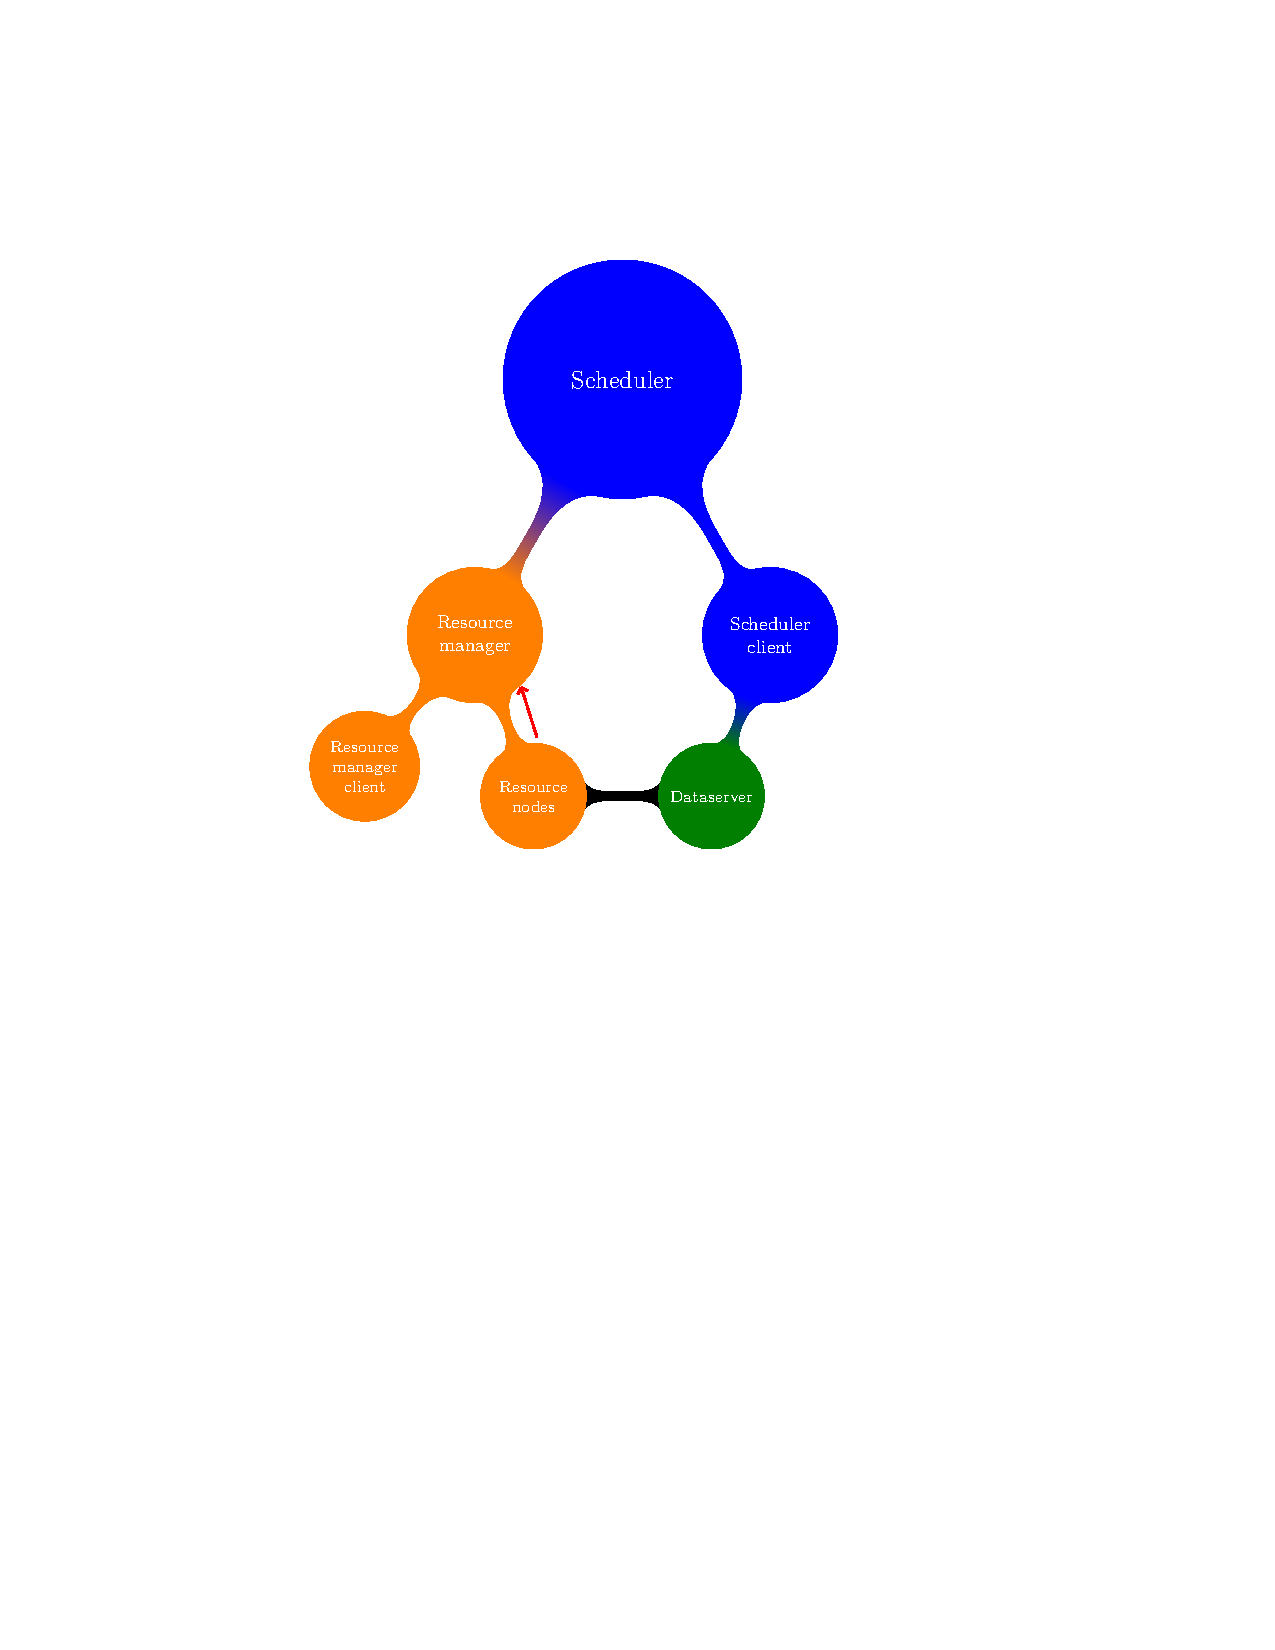
\includegraphics[trim=4cm 13cm 2cm 5cm,scale=0.48]{node_declaration.pdf}
            \caption{Communication dans Proactive}
        \end{figure}
	\end{column}
    \setbeamercolor{block title}{fg=black,bg=orange}   
    \setbeamercolor{block body}{fg=black,bg=orange!30}
    \setbeamercolor{block title alerted}{fg=black,bg=blue}   
    \setbeamercolor{block body alerted}{fg=black,bg=blue!30}
	\begin{column}[r]{0.5\linewidth}
        
        \begin{block}{Resource node}<1->
            \begin{itemize}
                \item À lancer sur chaque machine
                \item Reçoit les taches
                \item Les exécute dans un environnement temporaire
            \end{itemize}
        \end{block}
        \begin{block}{Resource manager}<2->
             Attend :
             \begin{itemize}
                     \item la connexion des resource nodes
                     \item les requêtes du scheduler
             \end{itemize}
        \end{block}
	\end{column}
	\end{columns}
\end{frame}

\begin{frame}{Dataserver}
	\begin{columns}
	\begin{column}[l]{0.5\linewidth}
        \begin{figure}
            %[!bh]
            \centering
            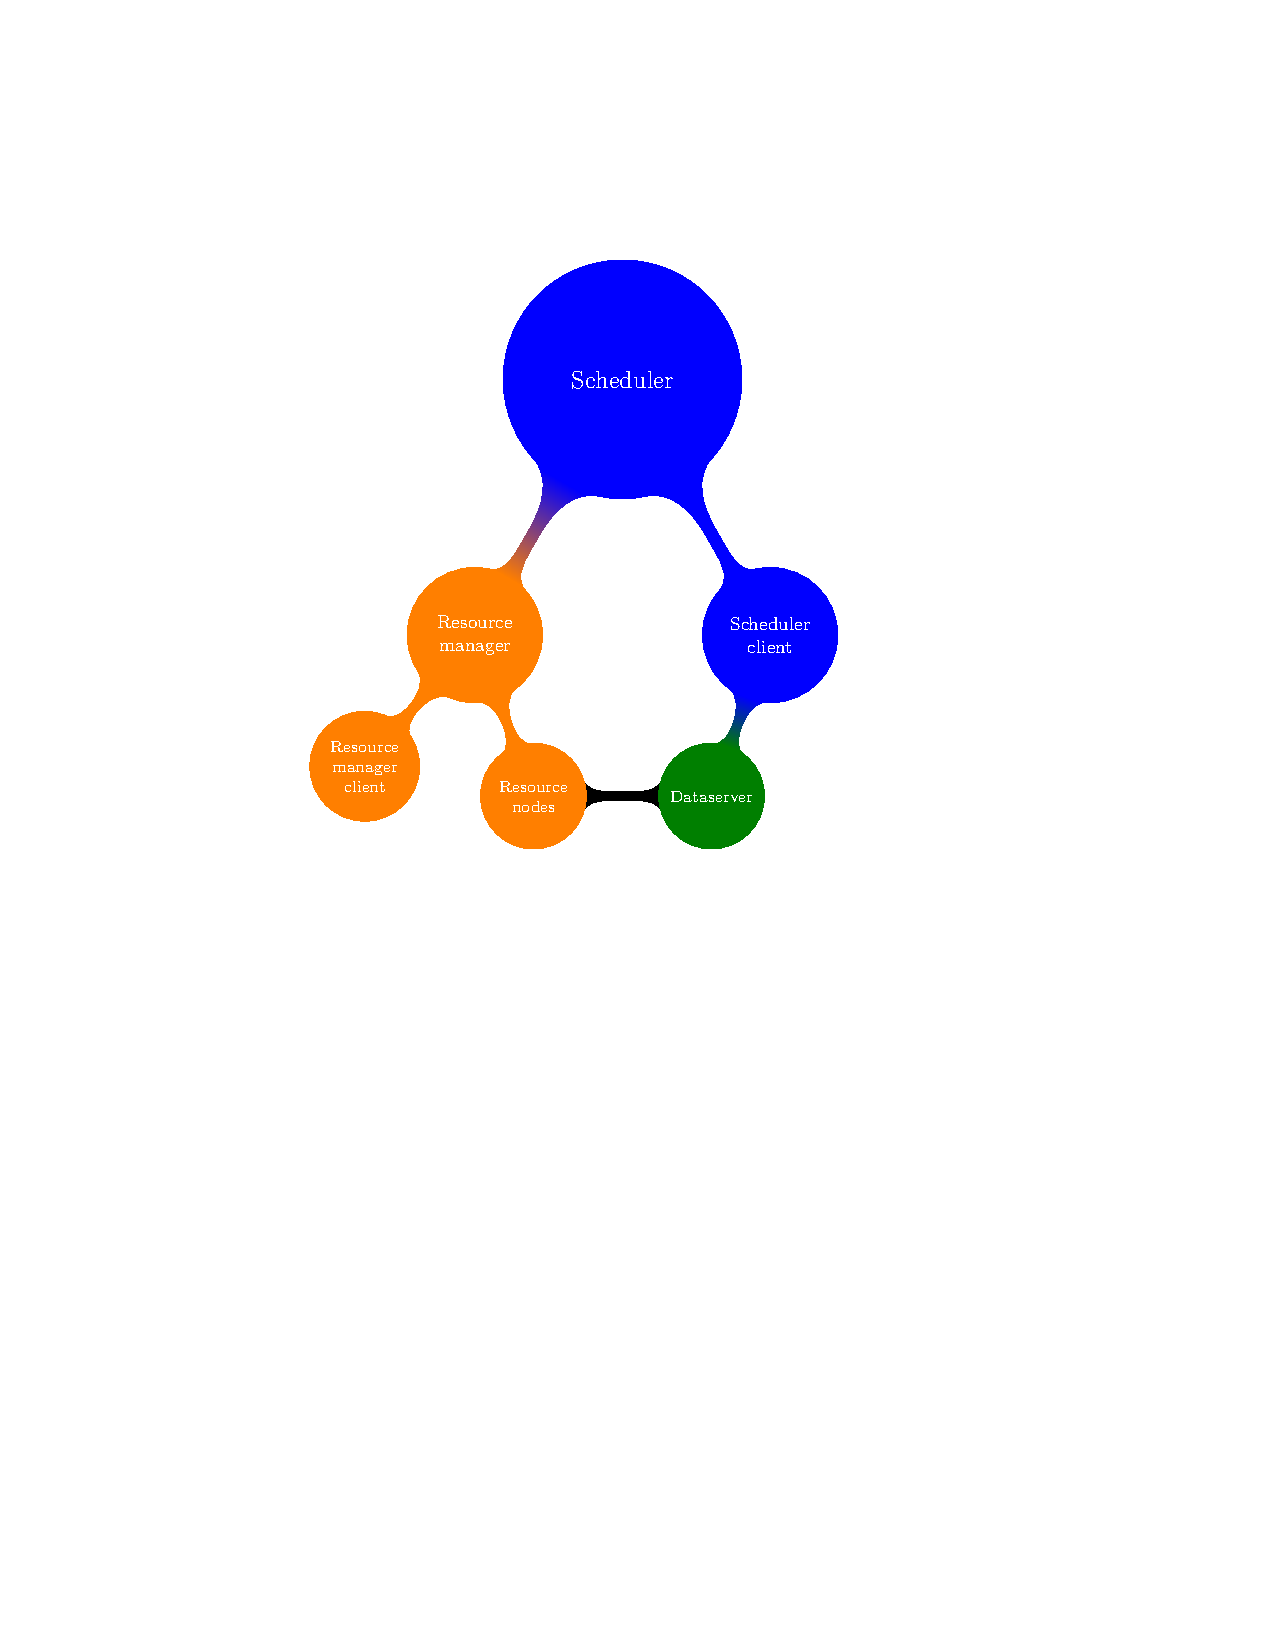
\includegraphics[trim=4cm 13cm 2cm 5cm,scale=0.48]{netmap_abs.pdf}
            \caption{Communication dans Proactive}
        \end{figure}
	\end{column}
    \setbeamercolor{block title example}{fg=black,bg=green!50!black}   
    \setbeamercolor{block body example}{fg=black,bg=green!15}
	\begin{column}[r]{0.5\linewidth}
        \begin{exampleblock}{Dataserver}
            \begin{itemize}
                \item Crée un espace accessible en lecture et en écriture

             %Peut être lancé par un administrateur pour fournir un espace permanent commun à tous les utilisateurs (faisable au CBGP, petite taille)
             %peut être lancé par chaque client pour créer l'espace sur sa propre machine
             \item Permanent et commun ou temporaire et personnel
             \item Espace partageable entre les clients et les t\^aches
             %Plusieurs client peuvent avoir accès au même espace
            \end{itemize}
            
        \end{exampleblock}
        
	\end{column}
	\end{columns}
    
\end{frame}

\begin{frame}{Scheduler (Ordonnanceur)}
	\begin{columns}
	\begin{column}[l]{0.5\linewidth}
        \only<1>{\begin{figure}
            %[!bh]
            \centering
            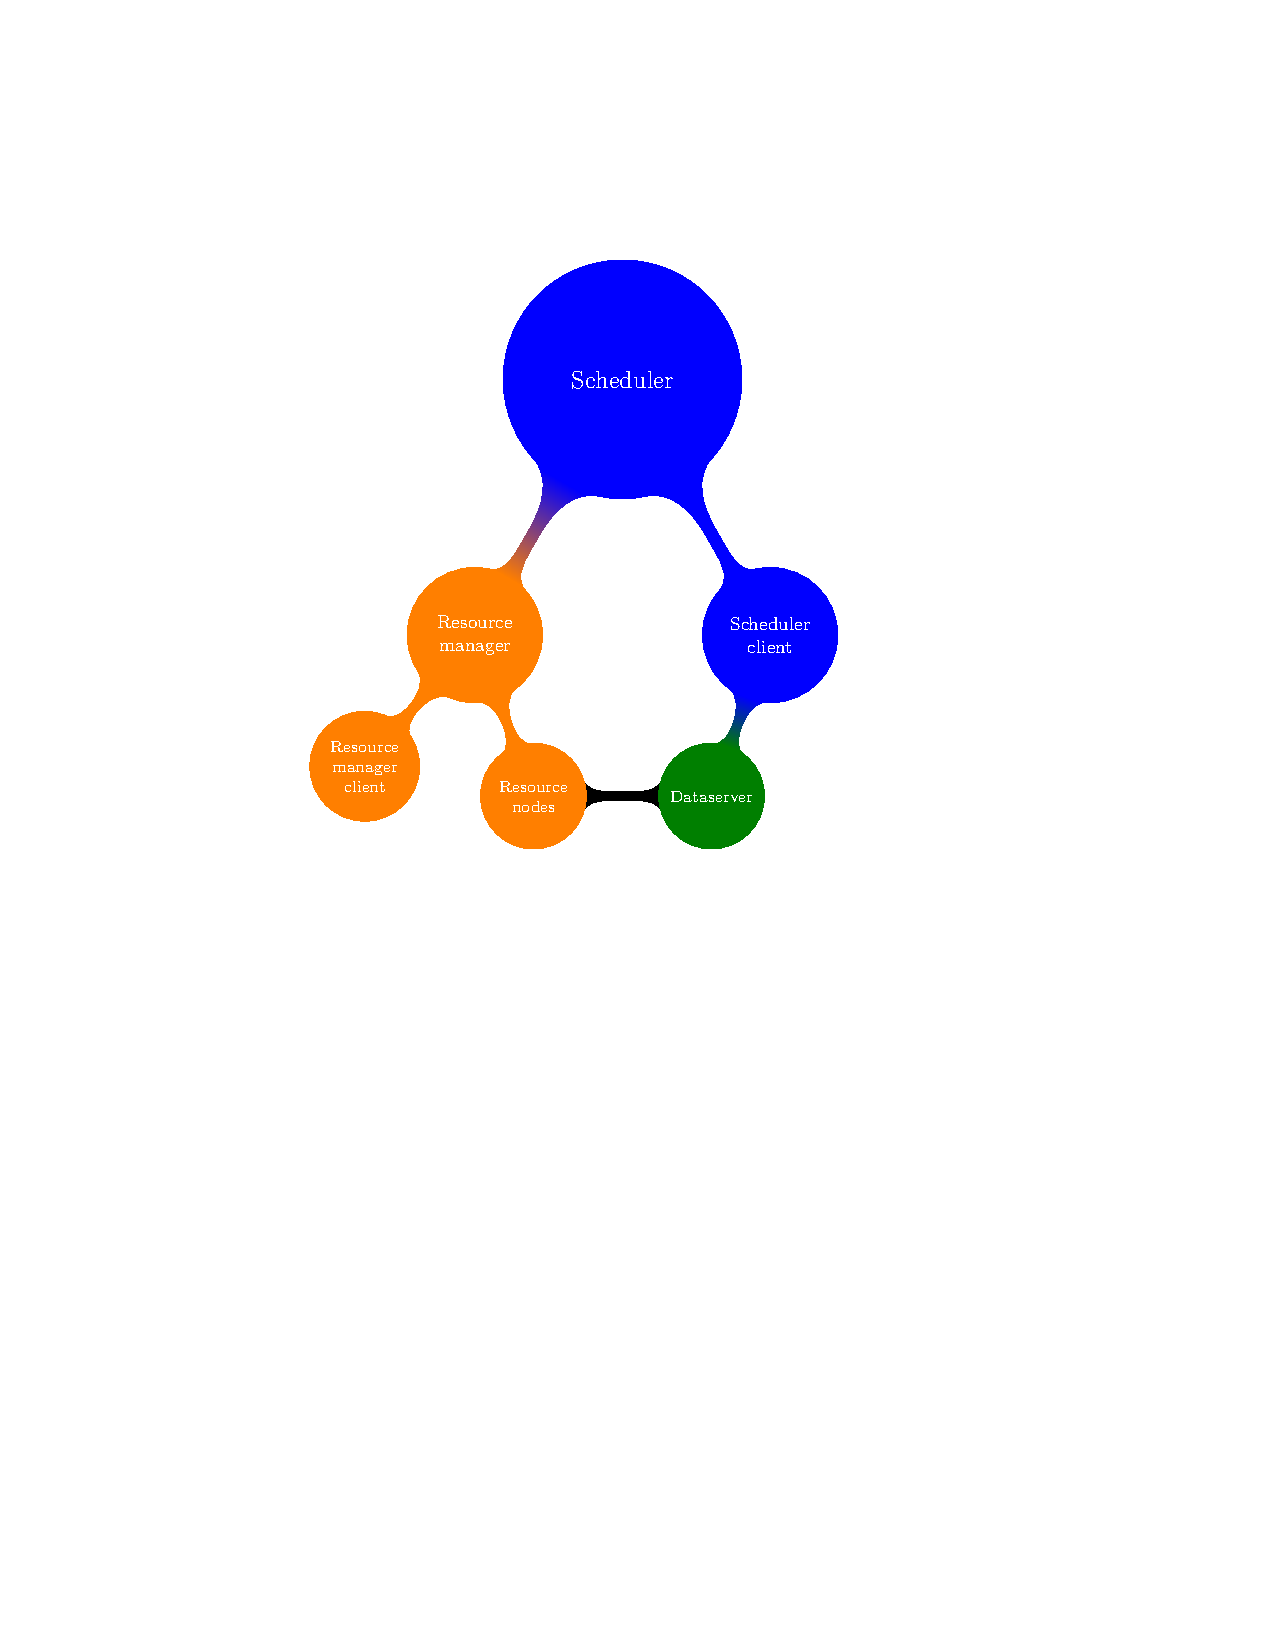
\includegraphics[trim=4cm 13cm 2cm 5cm,scale=0.48]{netmap_abs.pdf}
            \caption{Communication dans Proactive}
        \end{figure}}
        \only<2>{\begin{figure}
            %[!bh]
            \centering
            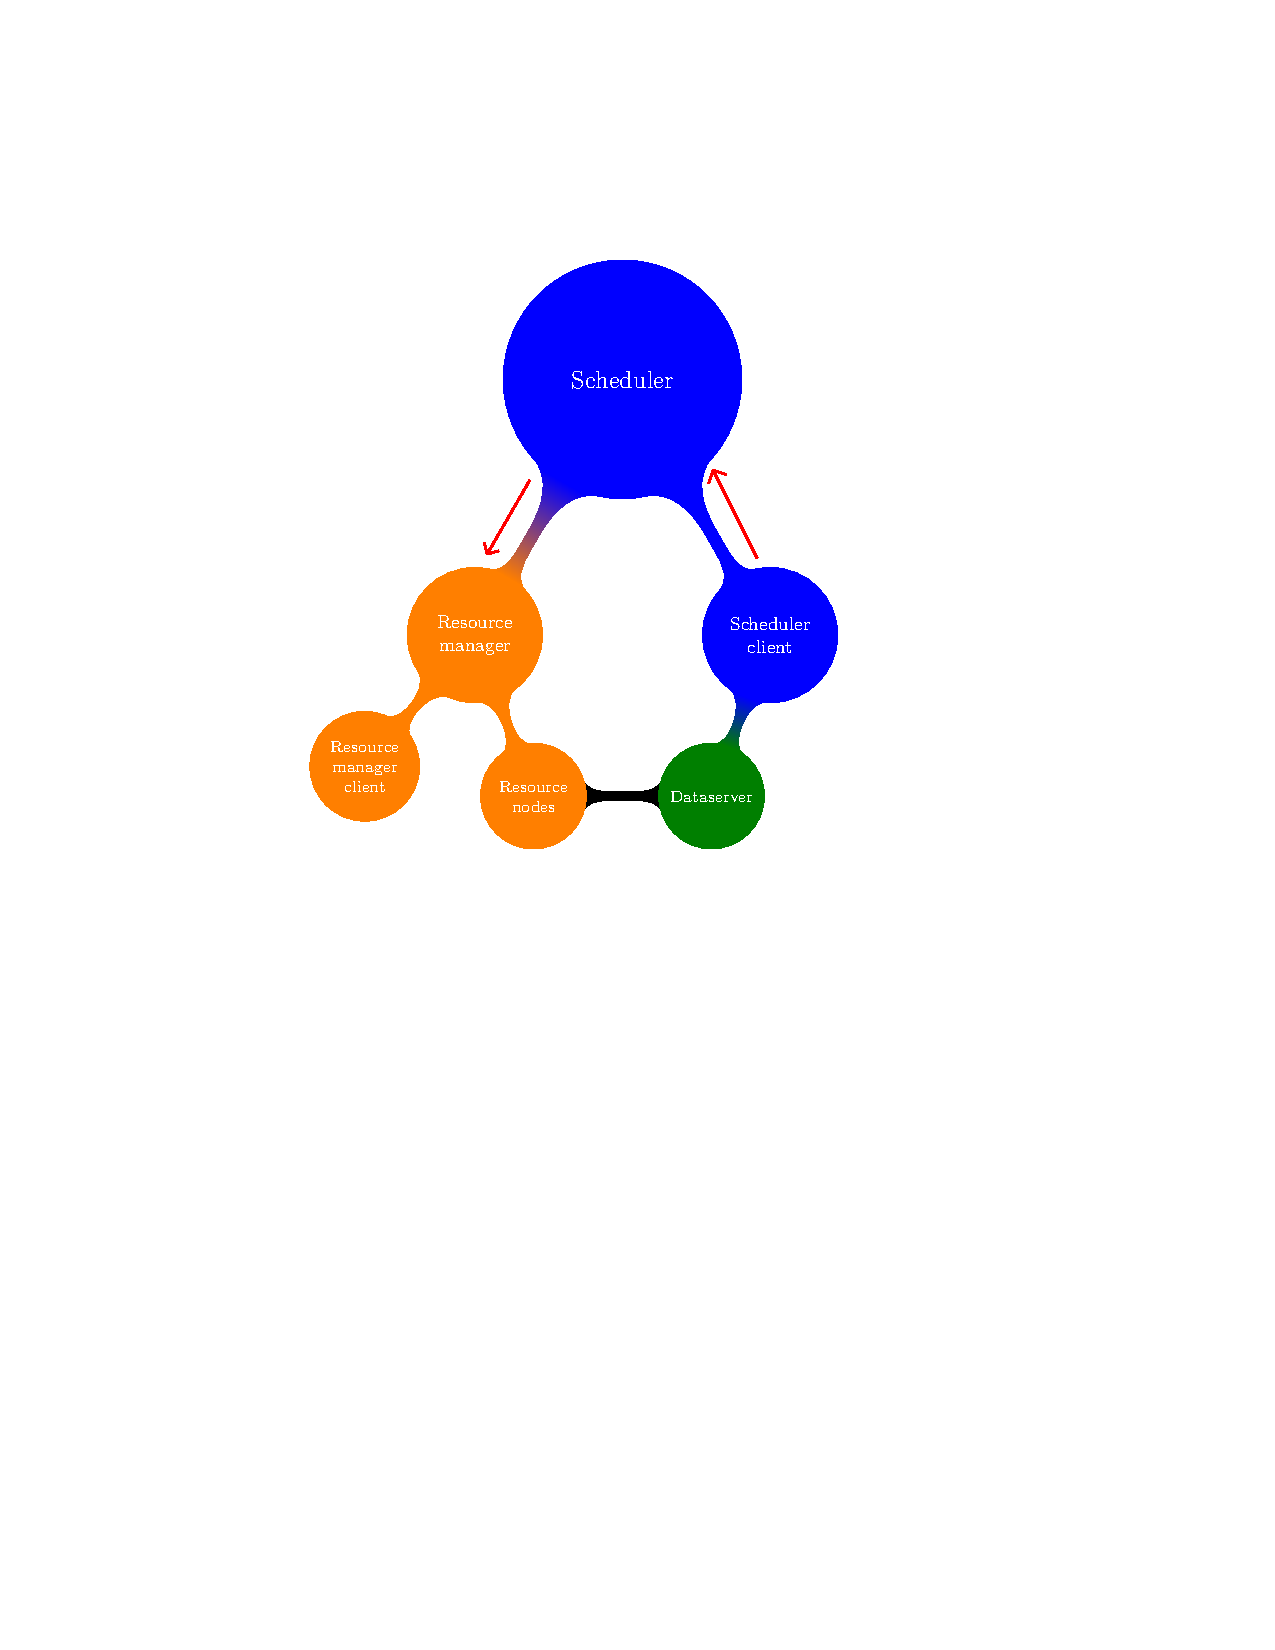
\includegraphics[trim=4cm 13cm 2cm 5cm,scale=0.48]{submit.pdf}
            \caption{Communication dans Proactive}
        \end{figure}}
        \only<3>{\begin{figure}
            %[!bh]
            \centering
            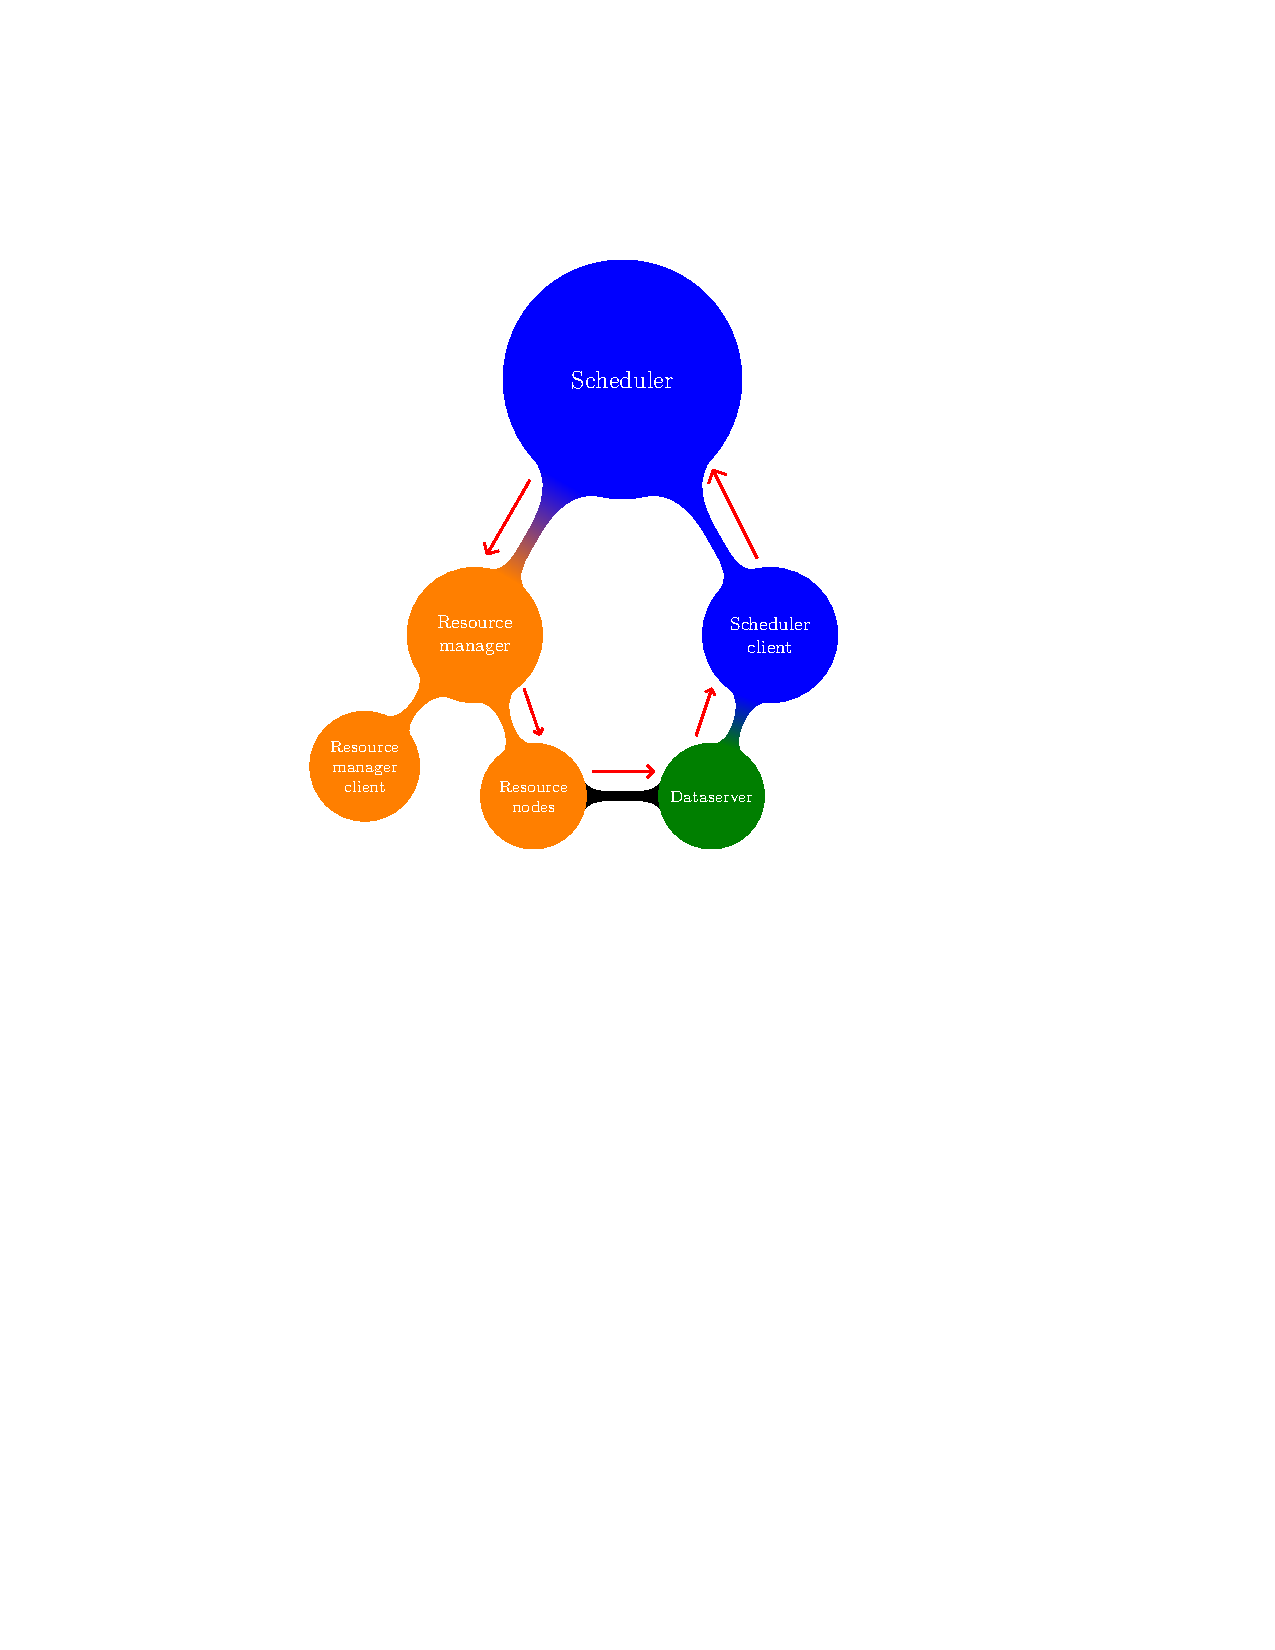
\includegraphics[trim=4cm 13cm 2cm 5cm,scale=0.48]{submit2.pdf}
            \caption{Communication dans Proactive}
        \end{figure}}
	\end{column}
    \setbeamercolor{block title}{fg=black,bg=blue}   
    \setbeamercolor{block body}{fg=black,bg=blue!30}
	\begin{column}[r]{0.5\linewidth}
        \only<1>{\begin{block}{Scheduler}
            \begin{itemize}
            \item Intermédiaire entre le client et le resource manager
            \item Authentification des clients 
            \item Droits d'accès aux ressources 
            \item Affectation des taches aux resource nodes
            \end{itemize}
        \end{block}}
        \only<2-3>{
        \begin{block}{Soumission d'un job}
            \begin{itemize}
            \item<2-> Transmission au scheduler
            \item<2-> Transmission au resource manager
            \item<3-> Affectation aux nodes
            \item<3-> Transmission des résultats
            \end{itemize}
        \end{block}
        }
        
	\end{column}
	\end{columns}
    
\end{frame}

%\subsection{Architecture}
%
%\begin{frame}{Communication dans Proactive}
%    \begin{figure}
%        %[!bh]
%        \centering
%        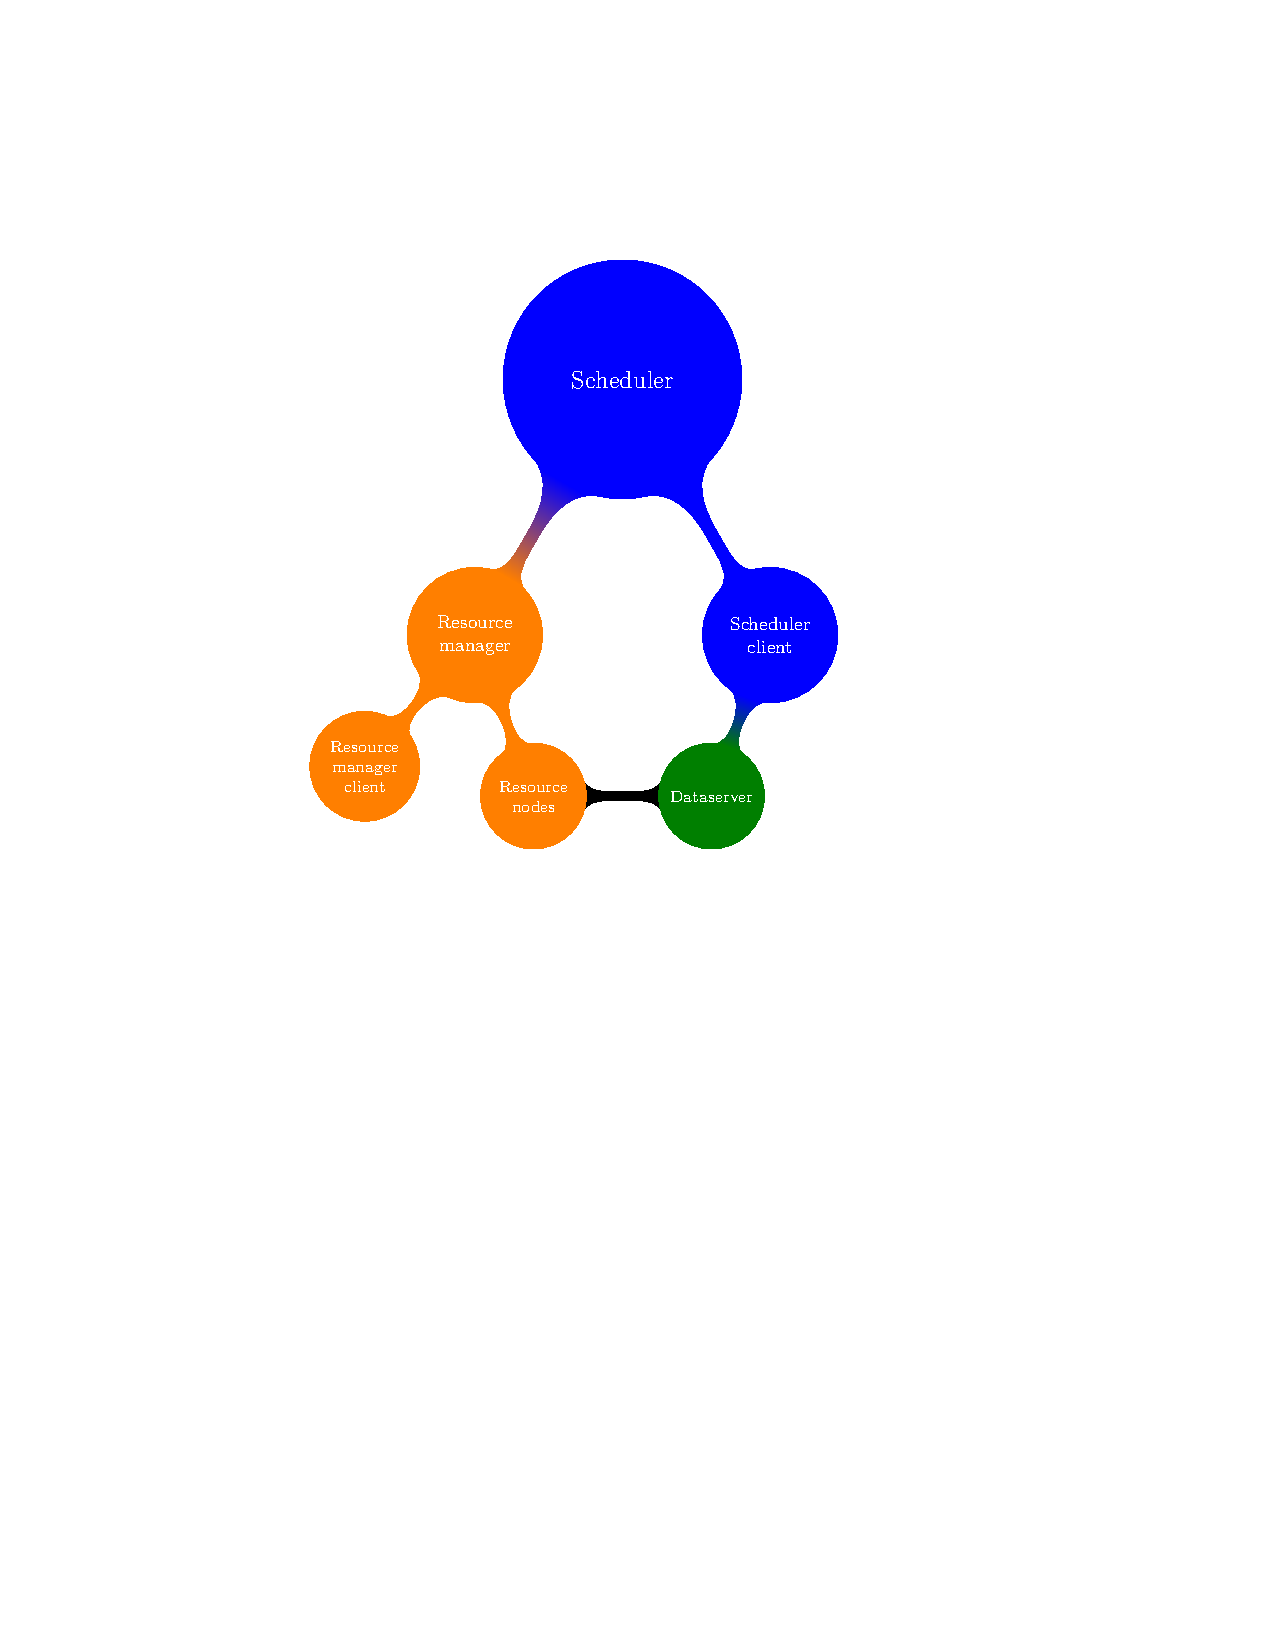
\includegraphics[trim=4cm 13cm 4cm 4cm,scale=0.62]{netmap_abs.pdf}
%        %\caption{Principe de communication dans le réseau Proactive}
%    \end{figure}
%    
%\end{frame}

\subsection{Définition d'une tache}
\begin{frame}
        \begin{block}{Qu'est-ce qu'une t\^ache ? (Job)}<1->
        % en java, par xml, ou par liste de commandes
            \begin{itemize}
                \item Un identifiant
                \item Un serveur de données
                \item Une liste d'opération à effectuer %option dependances, retry..
            \end{itemize}
        \end{block}
        \begin{exampleblock}{Quels sont les types de t\^ache ?}<2->
        % en java, par xml, ou par liste de commandes
            \begin{itemize}
                \item Native : Lance un script/binaire qui doit être compatible avec le noeud
                \item Java : transport et exécution d'un exécutable Java
            \end{itemize}
        \end{exampleblock}
        \begin{exampleblock}{Exemples d'options}<3->
            \begin{itemize}
                \item Job : Priority, inputSpace, outputSpace, variables
                \item Task : restartTaskOnError, inputFiles, outputFiles, depends, selectionScript
            \end{itemize}
        \end{exampleblock}
\end{frame}

\begin{frame}{Avec une liste de commandes natives}
	\begin{columns}
	\begin{column}[l]{0.4\linewidth}
        \begin{exampleblock}{liste}
            \begin{itemize}
                \item Liste de commandes qui seront exécutées directement sur un noeud de calcul
                \item Gestion basique
            \end{itemize}
        \end{exampleblock}
	\end{column}
	\begin{column}[r]{0.6\linewidth}
        /path/to/script\_1.sh arg1 arg2\newline
        /path/to/script\_2.sh arg3 arg4\newline
        /path/to/script\_3.sh arg5 arg6\newline
	\end{column}
	\end{columns}
    
\end{frame}
\begin{frame}{En XML}
	\begin{columns}
	\begin{column}[l]{0.4\linewidth}
        \begin{exampleblock}{Définition par XML}
            \begin{itemize}
                \item T\^aches natives ou Java
                \item Fichier XML qui spécifie chaque paramètre
                \item Plus simple mais moins complète que Java
                \item T\^aches natives ou Java
            \end{itemize}
        \end{exampleblock}
	\end{column}
	\begin{column}[r]{0.6\linewidth}
        \vspace{-1cm}
        \begin{figure}
            %[!bh]
            \centering
            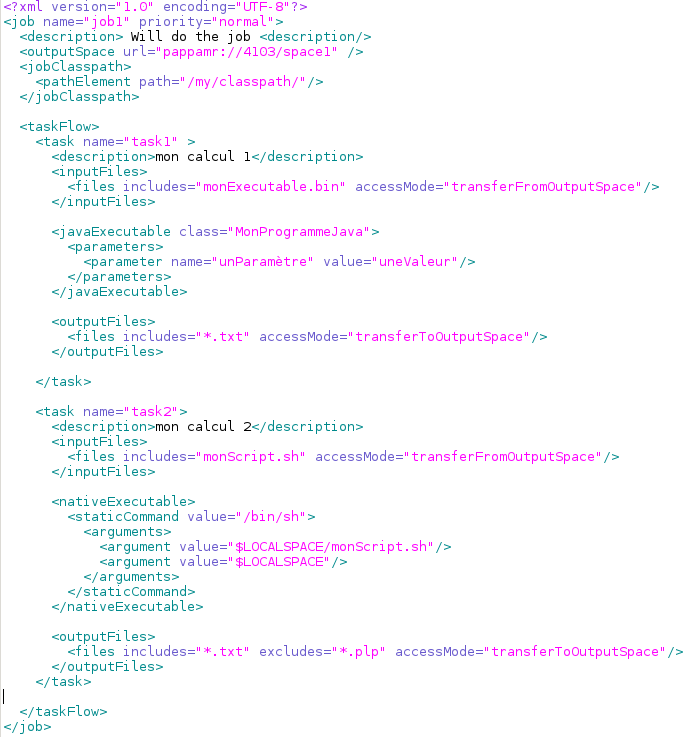
\includegraphics[scale=0.27]{jobxml.png}
            %\caption{Communication dans Proactive}
        \end{figure}
	\end{column}
	\end{columns}
    
\end{frame}
\begin{frame}{En Java}
	\begin{columns}
	\begin{column}[l]{0.4\linewidth}
        \begin{exampleblock}{Définition dans un programme en Java}
            \begin{itemize}
                \item Directement dans un programme en Java qui se connecte au scheduler
                \item Gestion fine
                \item T\^aches natives ou Java
            \end{itemize}
        \end{exampleblock}
	\end{column}
	\begin{column}[r]{0.6\linewidth}
        \vspace{-1cm}
        \begin{figure}
            %[!bh]
            \centering
            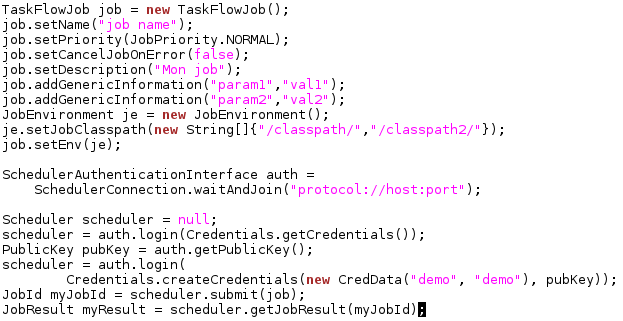
\includegraphics[scale=0.32]{jobjava.png}
            %\caption{Communication dans Proactive}
        \end{figure}
	\end{column}
	\end{columns}
    
\end{frame}

\subsection{Outils graphiques}
\begin{frame}{Scheduler client}
    % interessant pour la partie job submission et job results
    \begin{figure}
        %[!bh]
        \centering
        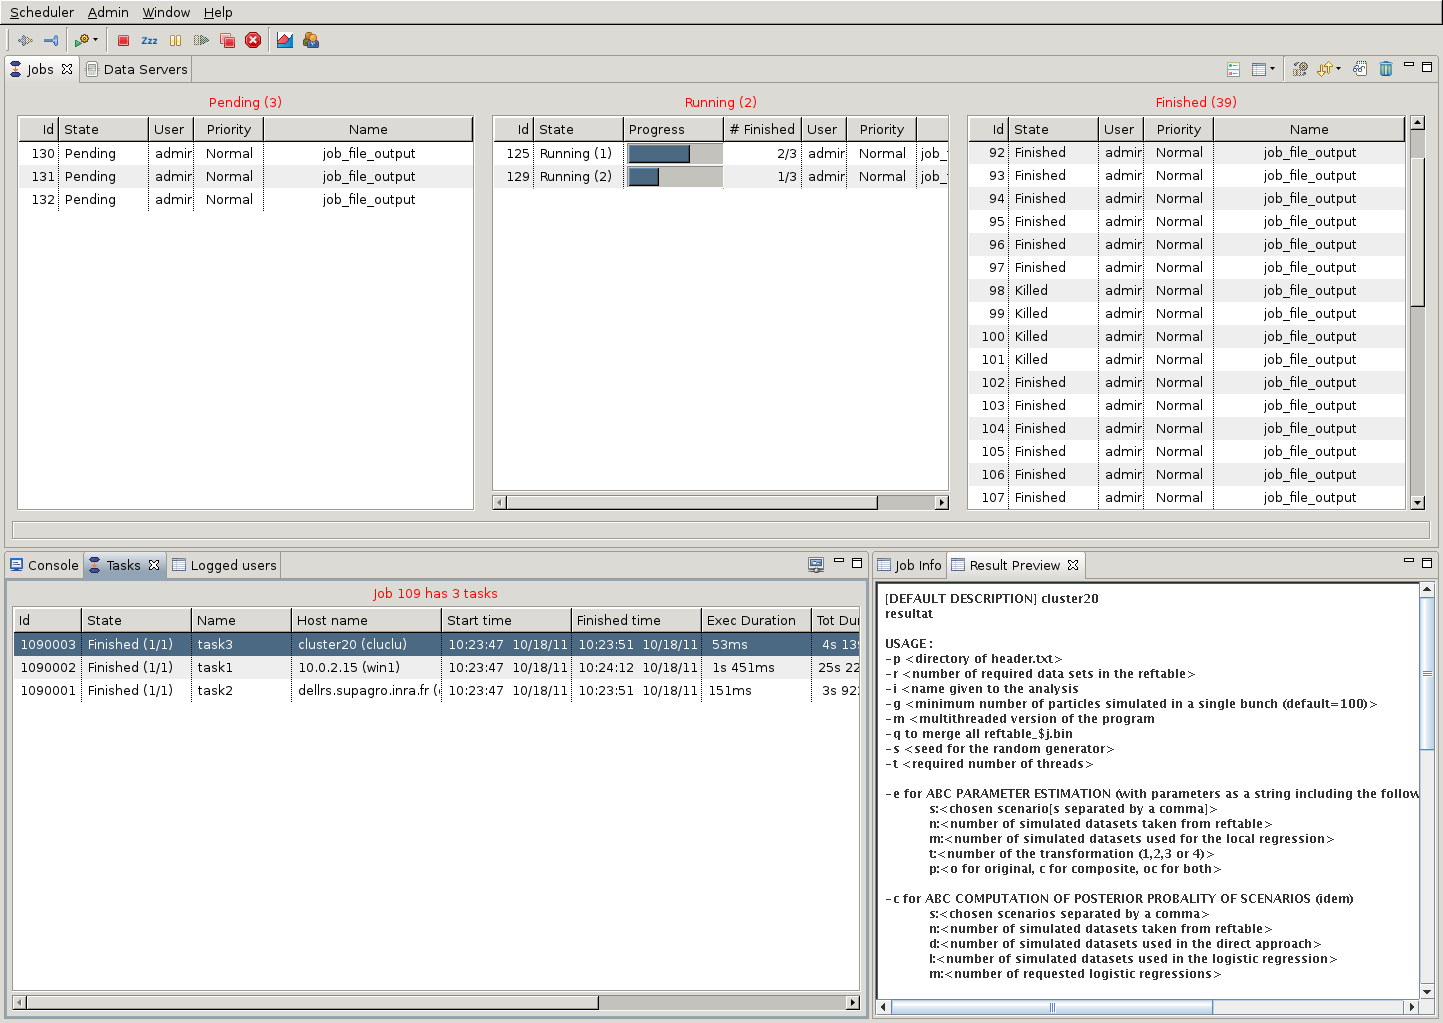
\includegraphics[scale=0.18]{sc_sched.png}
        %\caption{Principe de communication dans le réseau Proactive}
    \end{figure}
\end{frame}
\begin{frame}{Resource manager client}
    % interessant pour la partie monitoring
    \begin{figure}
        %[!bh]
        \centering
        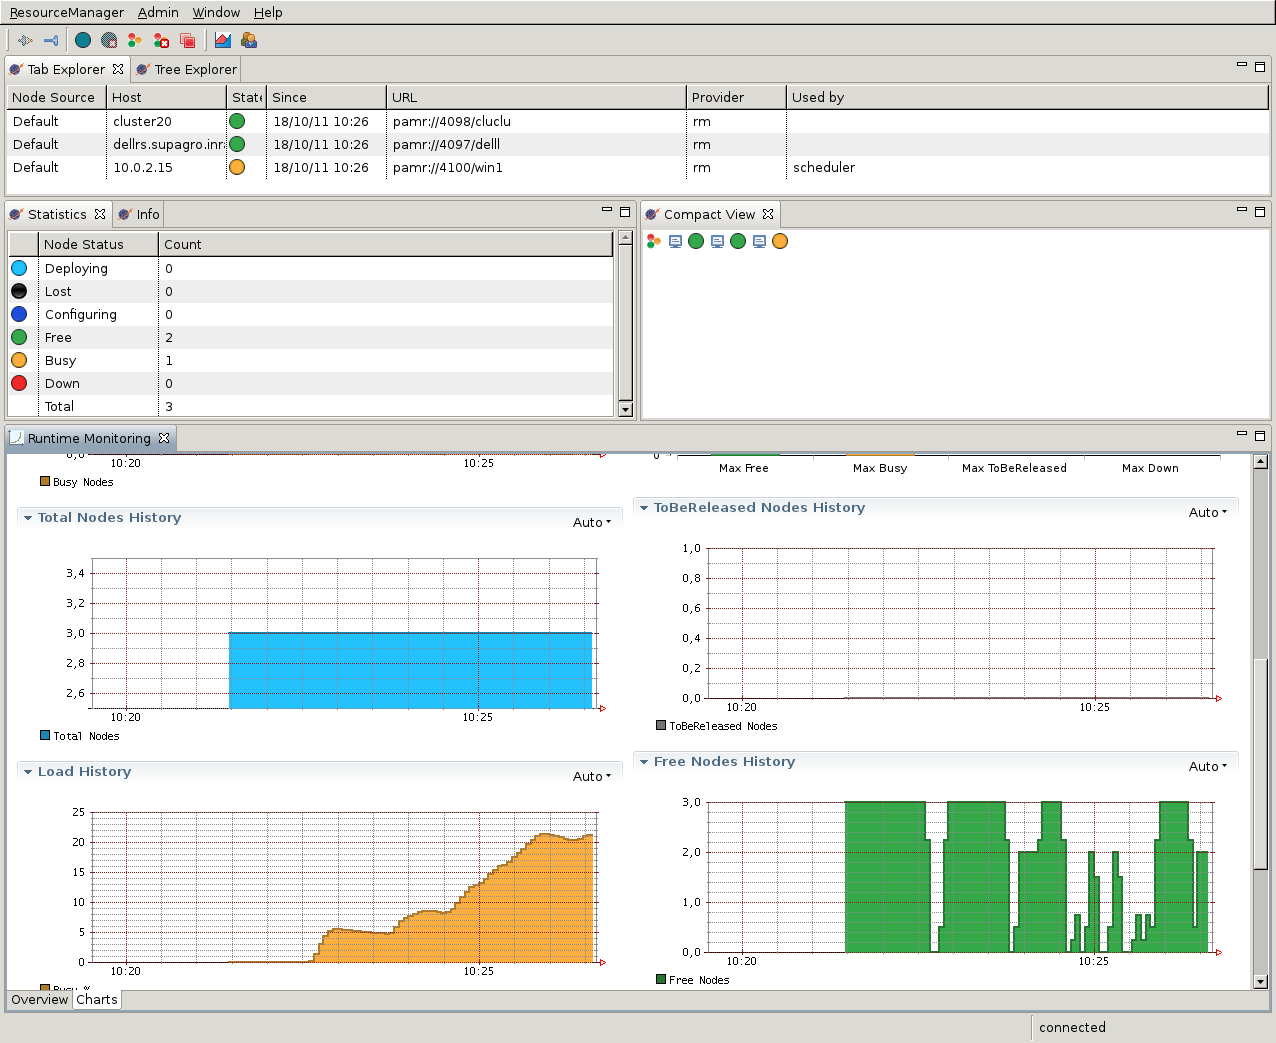
\includegraphics[scale=0.18]{sc_rmc.png}
        %\caption{Principe de communication dans le réseau Proactive}
    \end{figure}
\end{frame}


\section[Applications]{Applications possibles}
\begin{frame}
	\tableofcontents[currentsection]
\end{frame}
\subsection{Intégration avec un cluster}
\begin{frame}{Intégration des ressources d'un cluster existant}
    \setbeamercolor{block title}{fg=black,bg=violet}   
    \setbeamercolor{block body}{fg=black,bg=violet!10}
    \begin{block}{Protocoles}
    \begin{itemize}
        \item PBS (SGE, Torque \ldots)
        \item LSF
        \item SSH  
    \end{itemize}
        
    \end{block}
        \begin{figure}
            %[!bh]
            \centering
            \includegraphics[trim=1cm 13cm 2cm 4cm,scale=0.47]{res1.pdf}
            %\caption{}
        \end{figure}
\end{frame}
\subsection{Ressources individuelles}
\begin{frame}{Utiliser les postes de travail}
    \setbeamercolor{block title}{fg=black,bg=red!65!black}   
    \setbeamercolor{block body}{fg=black,bg=red!10}
    \begin{block}{Déployer manuellement des resource nodes}
    Avec le programme des noeuds de calcul
        
    \end{block}
    \begin{block}{PA-Agent}
    Programme d'automatisation de la mise à disposition des ressources
        
    \end{block}
    \vspace{0.2cm}
        \begin{figure}
            %[!bh]
            \centering
            \includegraphics[trim=4cm 13cm 2cm 5cm,scale=0.47]{res2.pdf}
            %\caption{}
        \end{figure}
\end{frame}
\subsection{Cloud}
\begin{frame}{Utiliser les ressources d'un cloud}
    \setbeamercolor{block title}{fg=black,bg=orange}   
    \setbeamercolor{block body}{fg=black,bg=orange!10}
    \vspace{-0.2cm}
    \only<1>{\begin{block}{Quels types de cloud ?}
        \begin{itemize}
            \item Amazon Elastic Compute Cloud (EC2)
            \item Windows High Performance Computing (HPC)
        \end{itemize}
    \end{block}}

    \only<2>{\begin{block}{Comment ?}
      %  Machine virtuelle dupliquée sur les noeuds du cloud qui lance 
     %On utilise la ressource dont on a besoin (pas plus pas moins) et seulement quand on en a besoin

     \begin{itemize}
         \item Déploiement par machines virtuelles
         \item Déploiement par outil interne 
     \end{itemize}
        
 \end{block}}

    \only<3>{\begin{block}{Avantages}
        \begin{itemize}
            \item Pas besoin d'avoir un cluster local, abstraction de l'architecture
            \item Utilisation sur mesure des ressources, investissement minimum % temporaire et la qtité qu'on veut
        \end{itemize}
    \end{block}}

        \begin{figure}
            %[!bh]
            \centering
            \includegraphics[trim=4cm 13cm 2cm 5cm,scale=0.47]{res3.pdf}
            %\caption{}
        \end{figure}
    
\end{frame}


\begin{frame}
	\begin{center}	{\huge Merci de votre attention}\end{center}
	\end{frame}
\begin{frame}
	\begin{center}	{\huge Questions}\end{center}
	\end{frame}

\end{document}
